\documentclass[../main.tex]{subfiles}

\begin{document}

\section{Annexes}
\label{sec:annexes}

\subsection{Tests d'interopérabilité}
\label{sec:interop}

Nous avons effectué des tests d'interopérabilité avec deux groupe : le groupe numéro 85 et le groupe numéro 93. 

Notre premier test a été réalisé avec le groupe 93. Lors de celui-ci, nous sommes parvenus à transférer des petits fichiers, et, ce, peu 
importe les arguments donnés au receiver (séquentiel, un seul \textit{handler}, etc.) sans aucun problème. Néanmoins, lors de plus gros transferts, 
des problèmes sont apparus.
Tout d'abord, il arrivait que notre receiver \textit{segfault}, ce qui, par ailleurs, entraînait un \textit{segfault} chez le \textit{sender}.
Une fois ce \textit{segfault} trouvé et corrigé, un \textit{livelock} avait l'air de se mettre en place de manière erratique, sauf lorsque 
notre receiver fonctionnait en mode séquentiel. Après analyse de la discussion \textit{sender} - \textit{receiver}, nous avons conclu
que ce comportement était le résultat du réordonnancement des paquets dû au multithreading du \textit{receiver} combiné avec la façon dont le 
\textit{sender} retransmettait sa \textit{window} en fonction du \textit{timestamp} des ACKs. Néanmoins, puisque le réordonnancement de paquets 
doit être supportée par le \textit{sender}, le problème était donc de leur côté. Par ailleurs nous avons aussi découvert que leur interprétation du 
champ \textit{window} était mauvaise. Ils avaient compris que ce champ indiquait la taille de notre \textit{window} et non l'espace restant dans celle-ci.

Notre deuxième test s'est passé de manière beaucoup plus fluide puisque le groupe 85 avait, comme nous, déjà corrigé les bugs d'interopérabilité.
Nous avons donc transmit nos fichiers sans aucun problèmes.

\subsection{Graphes partie critique}
\label{sec:graph_crit}

\newpage
\begin{figure}
    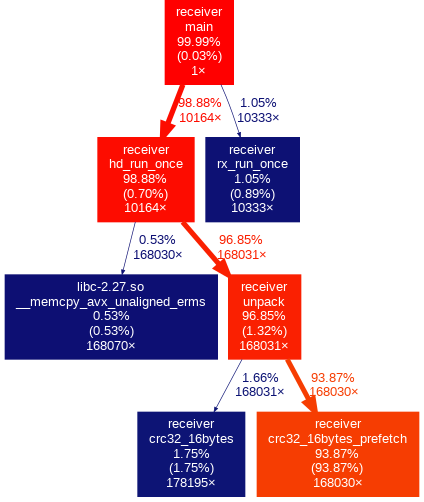
\includegraphics[scale=0.6]{assets/callgraph_seq.png}
    \caption{callgraph pour une exécution séquentielle}
\end{figure}

\newpage
\begin{figure}
    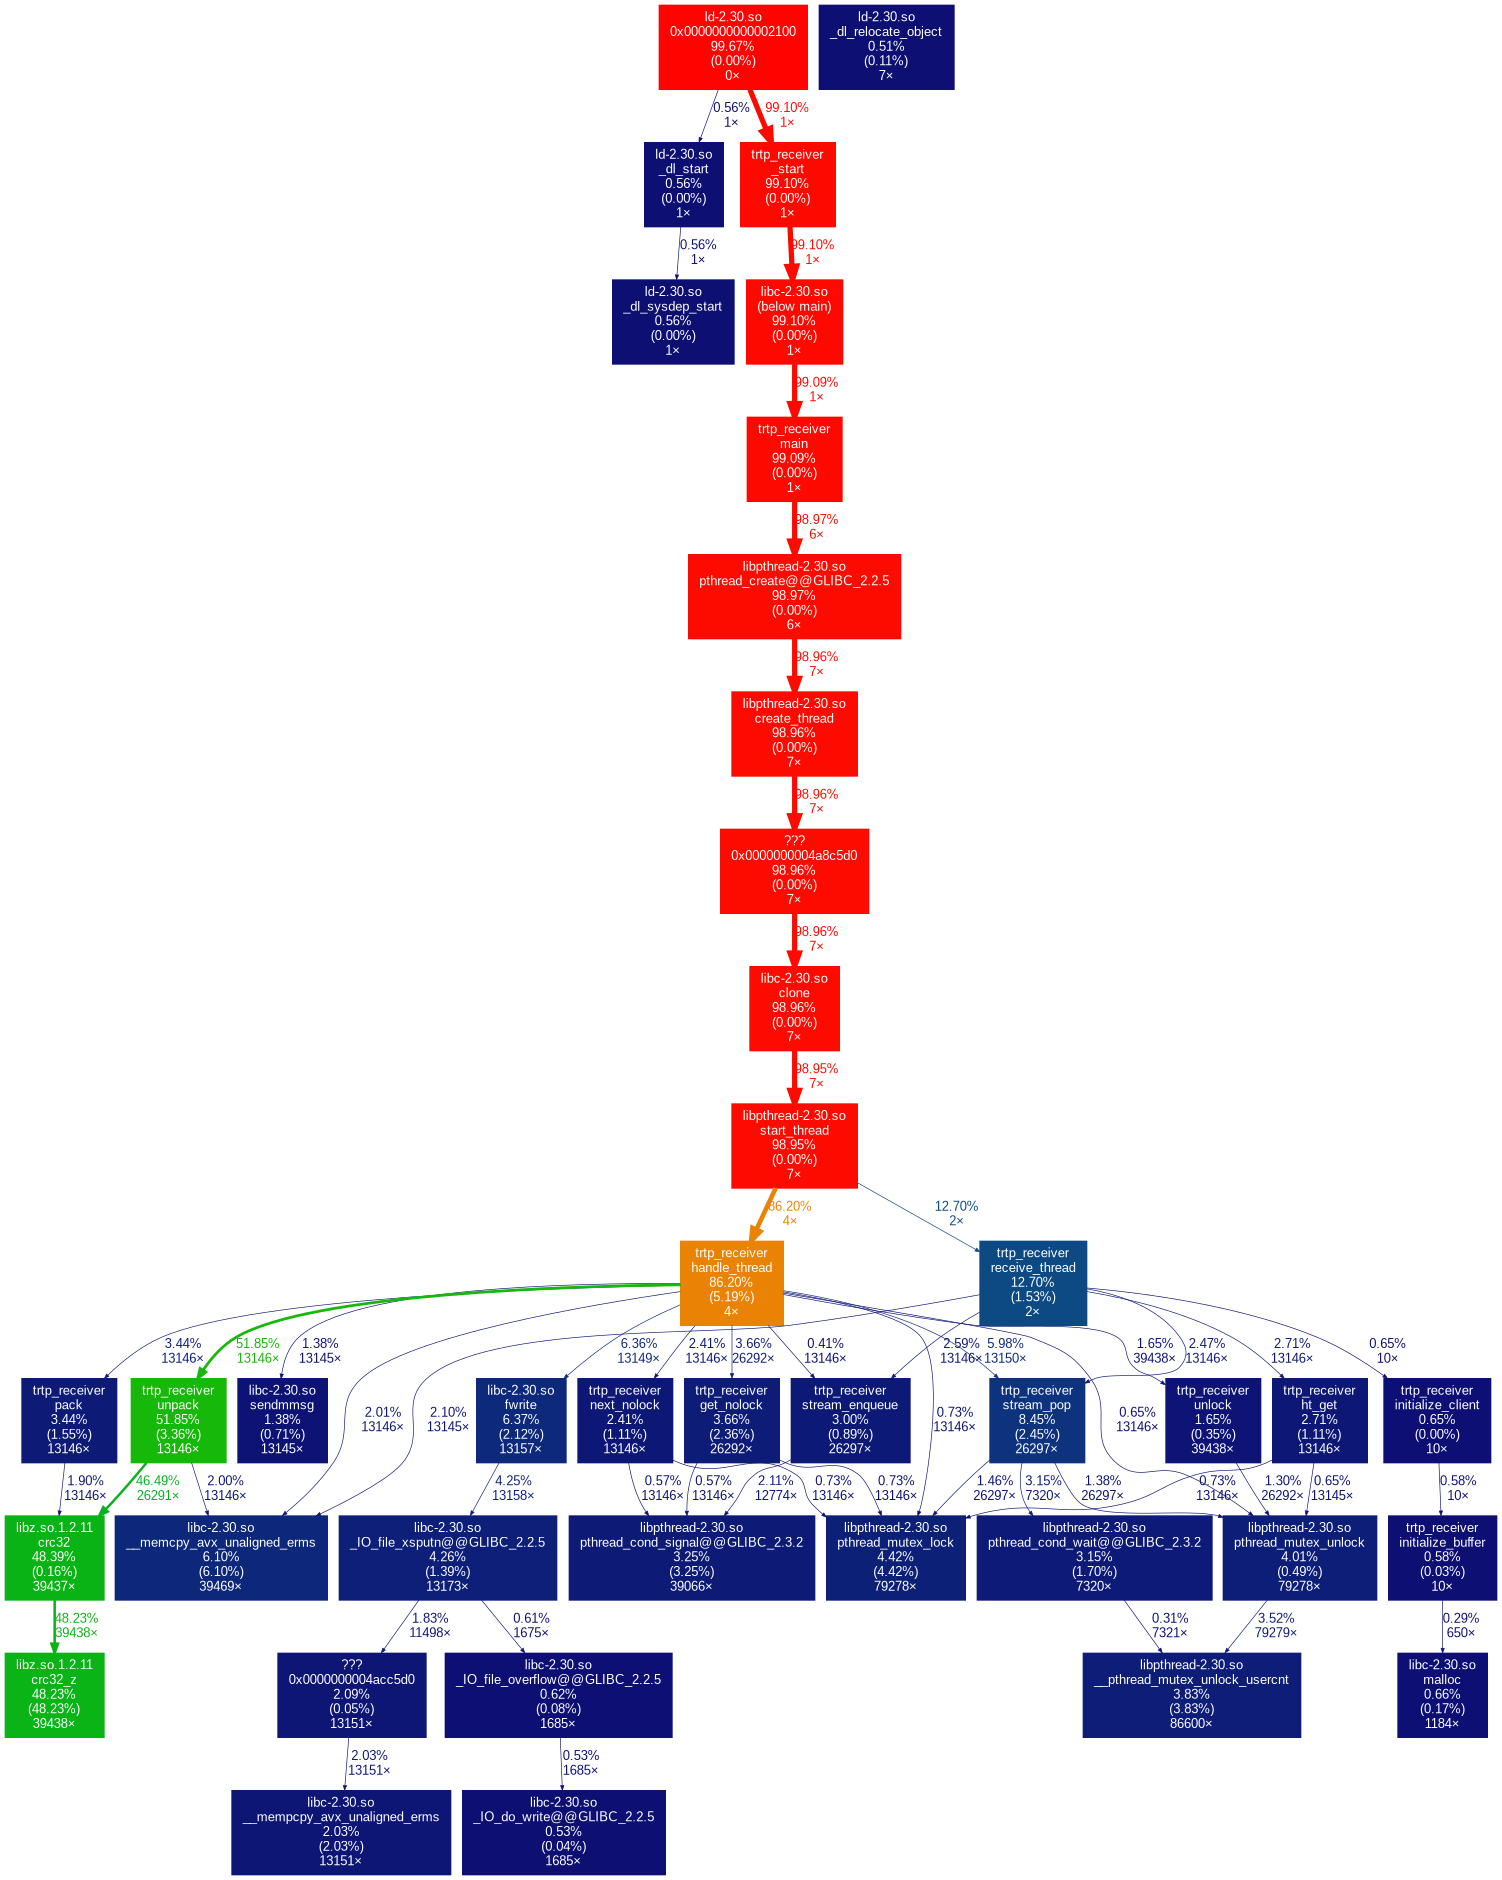
\includegraphics[scale=1.2]{assets/callgraph.png}
    \caption{callgraph pour une exécution multithreadée}
\end{figure}

\subsection{Comparaison des performances}

\label{sec:plot_1_recv}

\label{sec:plot_mul_recv}

\label{sec:plot_max}


\end{document}
